\documentclass[11pt]{article}
\usepackage[paper=letterpaper,margin=1in]{geometry}
\usepackage{mathtools}

\DeclarePairedDelimiter\ceil{\lceil}{\rceil}
\DeclarePairedDelimiter\floor{\lfloor}{\rfloor}
\usepackage[parfill]{parskip}
\usepackage{amsmath}
\usepackage{listings}
\usepackage{caption}
\usepackage[obeyspaces,spaces]{url}
\usepackage{graphicx}
\usepackage{tikz}
\usepackage{sourcecodepro}
\usepackage[T1]{fontenc}
\def\CC{{C\nolinebreak[4]\hspace{-.05em}\raisebox{.4ex}{\tiny\bf ++ }}}
\usepackage[
backend=biber,
citestyle=alphabetic,
style=alphabetic,
sorting=ynt
]{biblatex}
\lstset { %
    language=C++,
    backgroundcolor=\color{black!5}, % set backgroundcolor
    basicstyle=\ttfamily\footnotesize,% basic font setting
}
\addbibresource{sample.bib}
\DeclareUrlCommand\class{%
  \renewcommand{\UrlBigBreaks}{\do\.}%
  \renewcommand{\UrlBreaks}{\do\.}%
  }
\DeclareUrlCommand\filedir{%
  \renewcommand{\UrlBigBreaks}{\do\\}%
  \renewcommand{\UrlBreaks}{\do\\}%
  }
\DeclareUrlCommand\method{%
  \renewcommand{\UrlBigBreaks}{}%
  \renewcommand{\UrlBreaks}{}%
  }

\begin{document}
\thispagestyle{empty}
\title{Brief Analysis of Build Heap and Heapsort Algorithms \\
\large Assignment 406 \\
CS 310}
\date{April 6, 2017}
\author{Cameron Moberg}
\maketitle

A heap is a binary-tree-based data structure, where, depending on the type, the parent of a node is always bigger or always smaller than its children.
The former is called a \textit{max heap}; the latter a \textit{min heap}, and in this analysis we will exclusively be referring to a \textit{max heap}. We will also be analyzing methods that heaps are integral in: \method{build_heap} and \method{heap_sort}.

For both methods, the value for $n$ represents the number of nodes in the heap.

\section{Build Heap}
To analyze the \method{build_heap} algorithm, we chose the \method{percolate_down} algorithm on line 165 as the basic operation because it is called most frequently, is the most expensive, and is the philosophical heart of this algorithm. However, the runtime of  \method{percolate_down} is unknown and thus we must first analyze it to compute the time complexity of  \method{build_heap}.
\subsection{Percolate Down}

To analyze the \method{percolate_down} algorithm we chose both the comparison between child nodes on line 192 and the comparison between root value and the largest valued child node on line 200 as the basic operations. This is because they occur almost equally frequently and are the philosophical heart of this algorithm. Even though checking whether or not the node has children occurs most frequently, we didn't choose it as the basic operation because it's not the comparison we truly care about.

In this algorithm, we must assume that the root node's children are recursively heaps and then compare the root with both of its children. If any of the (at most 2) children are bigger in value than the root node, we swap values with the highest valued node, and then recursively use \method{percolate_down} on the node that was just swapped. We repeat this until the node is greater than or equal to its children or it is a leaf.
\clearpage

An empirical analysis of the \method{percolate_down} algorithm with multiple values of $n$ produces the results shown in Figure \ref{fig:perc}. The standard function $f(n) = \log n$ with a constant multiplier has been added to illustrate the analysis.

\begin{figure} [h]
\begin{center}
    % GNUPLOT: LaTeX picture with Postscript
\begingroup
  \makeatletter
  \providecommand\color[2][]{%
    \GenericError{(gnuplot) \space\space\space\@spaces}{%
      Package color not loaded in conjunction with
      terminal option `colourtext'%
    }{See the gnuplot documentation for explanation.%
    }{Either use 'blacktext' in gnuplot or load the package
      color.sty in LaTeX.}%
    \renewcommand\color[2][]{}%
  }%
  \providecommand\includegraphics[2][]{%
    \GenericError{(gnuplot) \space\space\space\@spaces}{%
      Package graphicx or graphics not loaded%
    }{See the gnuplot documentation for explanation.%
    }{The gnuplot epslatex terminal needs graphicx.sty or graphics.sty.}%
    \renewcommand\includegraphics[2][]{}%
  }%
  \providecommand\rotatebox[2]{#2}%
  \@ifundefined{ifGPcolor}{%
    \newif\ifGPcolor
    \GPcolorfalse
  }{}%
  \@ifundefined{ifGPblacktext}{%
    \newif\ifGPblacktext
    \GPblacktexttrue
  }{}%
  % define a \g@addto@macro without @ in the name:
  \let\gplgaddtomacro\g@addto@macro
  % define empty templates for all commands taking text:
  \gdef\gplbacktext{}%
  \gdef\gplfronttext{}%
  \makeatother
  \ifGPblacktext
    % no textcolor at all
    \def\colorrgb#1{}%
    \def\colorgray#1{}%
  \else
    % gray or color?
    \ifGPcolor
      \def\colorrgb#1{\color[rgb]{#1}}%
      \def\colorgray#1{\color[gray]{#1}}%
      \expandafter\def\csname LTw\endcsname{\color{white}}%
      \expandafter\def\csname LTb\endcsname{\color{black}}%
      \expandafter\def\csname LTa\endcsname{\color{black}}%
      \expandafter\def\csname LT0\endcsname{\color[rgb]{1,0,0}}%
      \expandafter\def\csname LT1\endcsname{\color[rgb]{0,1,0}}%
      \expandafter\def\csname LT2\endcsname{\color[rgb]{0,0,1}}%
      \expandafter\def\csname LT3\endcsname{\color[rgb]{1,0,1}}%
      \expandafter\def\csname LT4\endcsname{\color[rgb]{0,1,1}}%
      \expandafter\def\csname LT5\endcsname{\color[rgb]{1,1,0}}%
      \expandafter\def\csname LT6\endcsname{\color[rgb]{0,0,0}}%
      \expandafter\def\csname LT7\endcsname{\color[rgb]{1,0.3,0}}%
      \expandafter\def\csname LT8\endcsname{\color[rgb]{0.5,0.5,0.5}}%
    \else
      % gray
      \def\colorrgb#1{\color{black}}%
      \def\colorgray#1{\color[gray]{#1}}%
      \expandafter\def\csname LTw\endcsname{\color{white}}%
      \expandafter\def\csname LTb\endcsname{\color{black}}%
      \expandafter\def\csname LTa\endcsname{\color{black}}%
      \expandafter\def\csname LT0\endcsname{\color{black}}%
      \expandafter\def\csname LT1\endcsname{\color{black}}%
      \expandafter\def\csname LT2\endcsname{\color{black}}%
      \expandafter\def\csname LT3\endcsname{\color{black}}%
      \expandafter\def\csname LT4\endcsname{\color{black}}%
      \expandafter\def\csname LT5\endcsname{\color{black}}%
      \expandafter\def\csname LT6\endcsname{\color{black}}%
      \expandafter\def\csname LT7\endcsname{\color{black}}%
      \expandafter\def\csname LT8\endcsname{\color{black}}%
    \fi
  \fi
    \setlength{\unitlength}{0.0500bp}%
    \ifx\gptboxheight\undefined%
      \newlength{\gptboxheight}%
      \newlength{\gptboxwidth}%
      \newsavebox{\gptboxtext}%
    \fi%
    \setlength{\fboxrule}{0.5pt}%
    \setlength{\fboxsep}{1pt}%
\begin{picture}(7200.00,5040.00)%
    \gplgaddtomacro\gplbacktext{%
      \csname LTb\endcsname%
      \put(682,704){\makebox(0,0)[r]{\strut{}$0$}}%
      \put(682,1623){\makebox(0,0)[r]{\strut{}$5$}}%
      \put(682,2542){\makebox(0,0)[r]{\strut{}$10$}}%
      \put(682,3460){\makebox(0,0)[r]{\strut{}$15$}}%
      \put(682,4379){\makebox(0,0)[r]{\strut{}$20$}}%
      \put(1402,484){\makebox(0,0){\strut{}$500$}}%
      \put(2002,484){\makebox(0,0){\strut{}$1000$}}%
      \put(2602,484){\makebox(0,0){\strut{}$1500$}}%
      \put(3202,484){\makebox(0,0){\strut{}$2000$}}%
      \put(3802,484){\makebox(0,0){\strut{}$2500$}}%
      \put(4403,484){\makebox(0,0){\strut{}$3000$}}%
      \put(5003,484){\makebox(0,0){\strut{}$3500$}}%
      \put(5603,484){\makebox(0,0){\strut{}$4000$}}%
      \put(6203,484){\makebox(0,0){\strut{}$4500$}}%
      \put(6803,484){\makebox(0,0){\strut{}$5000$}}%
      \put(3202,3800){\rotatebox{7}{\makebox(0,0)[l]{\strut{}$\frac{3}{2} \log(n)$}}}%
    }%
    \gplgaddtomacro\gplfronttext{%
      \csname LTb\endcsname%
      \put(176,2541){\rotatebox{-270}{\makebox(0,0){\strut{}Operation Count}}}%
      \put(3808,154){\makebox(0,0){\strut{}Input Size}}%
      \put(3808,4709){\makebox(0,0){\strut{}Empirical Analysis of Percolate Down Algorithm}}%
    }%
    \gplbacktext
    \put(0,0){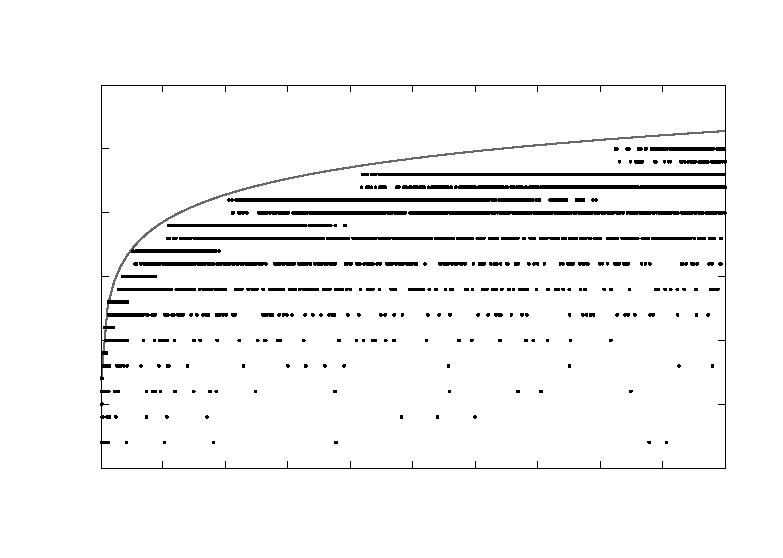
\includegraphics{perc}}%
    \gplfronttext
  \end{picture}%
\endgroup

    \caption{\small \sl Results of percolate down algorithm.\label{fig:perc}}  

\end{center}
\end{figure}
The \CC method used to produce Figure \ref{fig:perc} is shown below.

\begin{lstlisting}
    void empiric_perc( Comparable key )
    {
        heap.at( 0 ) = key; 	  //heap is a max_heap by definition.
        heap.percolate_down( 0 ); //0 is the root node index.
    }
\end{lstlisting}

In short, we set $key$ to a generated (pseudo) random number, set the root node of the heap equal to it, and then \method{percolate_down} is used on the root node to to simulate a ``worst-case scenario''.

An examination of the \method{percolate_down} implementation explains the empirical results when we observe that, in the worst-case, the root node's value is the smallest of all nodes in the tree. This means the node has to sift down through every level of the tree and become a leaf, at the bottom of the tree. This requires a comparison at every level, or, $\log n$ comparisons \cite{anal}.

Since this algorithm can terminate prematurely, we cannot tighten the bound to Big-$\Theta$, and thus the \method{percolate_down} algorithm can be described as 

\[
T(n) \in O( \log n)
\]
\[
T(n) \in \Omega(1)
\]
\clearpage
\subsection{Build Heap cont.}

An empirical analysis of running \method{build_heap()} with multiple values of $n$ produces the results shown in Figure \ref{fig:build}. The standard function $f(n) = n$ with constant multipliers has been added to further illustrate the analysis.
\begin{figure}[h]
\begin{center}
    % GNUPLOT: LaTeX picture with Postscript
\begingroup
  \makeatletter
  \providecommand\color[2][]{%
    \GenericError{(gnuplot) \space\space\space\@spaces}{%
      Package color not loaded in conjunction with
      terminal option `colourtext'%
    }{See the gnuplot documentation for explanation.%
    }{Either use 'blacktext' in gnuplot or load the package
      color.sty in LaTeX.}%
    \renewcommand\color[2][]{}%
  }%
  \providecommand\includegraphics[2][]{%
    \GenericError{(gnuplot) \space\space\space\@spaces}{%
      Package graphicx or graphics not loaded%
    }{See the gnuplot documentation for explanation.%
    }{The gnuplot epslatex terminal needs graphicx.sty or graphics.sty.}%
    \renewcommand\includegraphics[2][]{}%
  }%
  \providecommand\rotatebox[2]{#2}%
  \@ifundefined{ifGPcolor}{%
    \newif\ifGPcolor
    \GPcolorfalse
  }{}%
  \@ifundefined{ifGPblacktext}{%
    \newif\ifGPblacktext
    \GPblacktexttrue
  }{}%
  % define a \g@addto@macro without @ in the name:
  \let\gplgaddtomacro\g@addto@macro
  % define empty templates for all commands taking text:
  \gdef\gplbacktext{}%
  \gdef\gplfronttext{}%
  \makeatother
  \ifGPblacktext
    % no textcolor at all
    \def\colorrgb#1{}%
    \def\colorgray#1{}%
  \else
    % gray or color?
    \ifGPcolor
      \def\colorrgb#1{\color[rgb]{#1}}%
      \def\colorgray#1{\color[gray]{#1}}%
      \expandafter\def\csname LTw\endcsname{\color{white}}%
      \expandafter\def\csname LTb\endcsname{\color{black}}%
      \expandafter\def\csname LTa\endcsname{\color{black}}%
      \expandafter\def\csname LT0\endcsname{\color[rgb]{1,0,0}}%
      \expandafter\def\csname LT1\endcsname{\color[rgb]{0,1,0}}%
      \expandafter\def\csname LT2\endcsname{\color[rgb]{0,0,1}}%
      \expandafter\def\csname LT3\endcsname{\color[rgb]{1,0,1}}%
      \expandafter\def\csname LT4\endcsname{\color[rgb]{0,1,1}}%
      \expandafter\def\csname LT5\endcsname{\color[rgb]{1,1,0}}%
      \expandafter\def\csname LT6\endcsname{\color[rgb]{0,0,0}}%
      \expandafter\def\csname LT7\endcsname{\color[rgb]{1,0.3,0}}%
      \expandafter\def\csname LT8\endcsname{\color[rgb]{0.5,0.5,0.5}}%
    \else
      % gray
      \def\colorrgb#1{\color{black}}%
      \def\colorgray#1{\color[gray]{#1}}%
      \expandafter\def\csname LTw\endcsname{\color{white}}%
      \expandafter\def\csname LTb\endcsname{\color{black}}%
      \expandafter\def\csname LTa\endcsname{\color{black}}%
      \expandafter\def\csname LT0\endcsname{\color{black}}%
      \expandafter\def\csname LT1\endcsname{\color{black}}%
      \expandafter\def\csname LT2\endcsname{\color{black}}%
      \expandafter\def\csname LT3\endcsname{\color{black}}%
      \expandafter\def\csname LT4\endcsname{\color{black}}%
      \expandafter\def\csname LT5\endcsname{\color{black}}%
      \expandafter\def\csname LT6\endcsname{\color{black}}%
      \expandafter\def\csname LT7\endcsname{\color{black}}%
      \expandafter\def\csname LT8\endcsname{\color{black}}%
    \fi
  \fi
    \setlength{\unitlength}{0.0500bp}%
    \ifx\gptboxheight\undefined%
      \newlength{\gptboxheight}%
      \newlength{\gptboxwidth}%
      \newsavebox{\gptboxtext}%
    \fi%
    \setlength{\fboxrule}{0.5pt}%
    \setlength{\fboxsep}{1pt}%
\begin{picture}(7200.00,5040.00)%
    \gplgaddtomacro\gplbacktext{%
      \csname LTb\endcsname%
      \put(1078,704){\makebox(0,0)[r]{\strut{}$0$}}%
      \put(1078,1072){\makebox(0,0)[r]{\strut{}$1000$}}%
      \put(1078,1439){\makebox(0,0)[r]{\strut{}$2000$}}%
      \put(1078,1807){\makebox(0,0)[r]{\strut{}$3000$}}%
      \put(1078,2174){\makebox(0,0)[r]{\strut{}$4000$}}%
      \put(1078,2542){\makebox(0,0)[r]{\strut{}$5000$}}%
      \put(1078,2909){\makebox(0,0)[r]{\strut{}$6000$}}%
      \put(1078,3277){\makebox(0,0)[r]{\strut{}$7000$}}%
      \put(1078,3644){\makebox(0,0)[r]{\strut{}$8000$}}%
      \put(1078,4012){\makebox(0,0)[r]{\strut{}$9000$}}%
      \put(1078,4379){\makebox(0,0)[r]{\strut{}$10000$}}%
      \put(1210,484){\makebox(0,0){\strut{}$0$}}%
      \put(1769,484){\makebox(0,0){\strut{}$500$}}%
      \put(2329,484){\makebox(0,0){\strut{}$1000$}}%
      \put(2888,484){\makebox(0,0){\strut{}$1500$}}%
      \put(3447,484){\makebox(0,0){\strut{}$2000$}}%
      \put(4007,484){\makebox(0,0){\strut{}$2500$}}%
      \put(4566,484){\makebox(0,0){\strut{}$3000$}}%
      \put(5125,484){\makebox(0,0){\strut{}$3500$}}%
      \put(5684,484){\makebox(0,0){\strut{}$4000$}}%
      \put(6244,484){\makebox(0,0){\strut{}$4500$}}%
      \put(6803,484){\makebox(0,0){\strut{}$5000$}}%
      \put(2888,1929){\rotatebox{37}{\makebox(0,0)[l]{\strut{}$2n$}}}%
      \put(3447,1750){\rotatebox{33}{\makebox(0,0)[l]{\strut{}$\frac{7}{8} n$}}}%
    }%
    \gplgaddtomacro\gplfronttext{%
      \csname LTb\endcsname%
      \put(176,2541){\rotatebox{-270}{\makebox(0,0){\strut{}Operation Count}}}%
      \put(4006,154){\makebox(0,0){\strut{}Input Size}}%
      \put(4006,4709){\makebox(0,0){\strut{}\textbf{Empirical Analysis of Build Heap Algorithm}}}%
    }%
    \gplbacktext
    \put(0,0){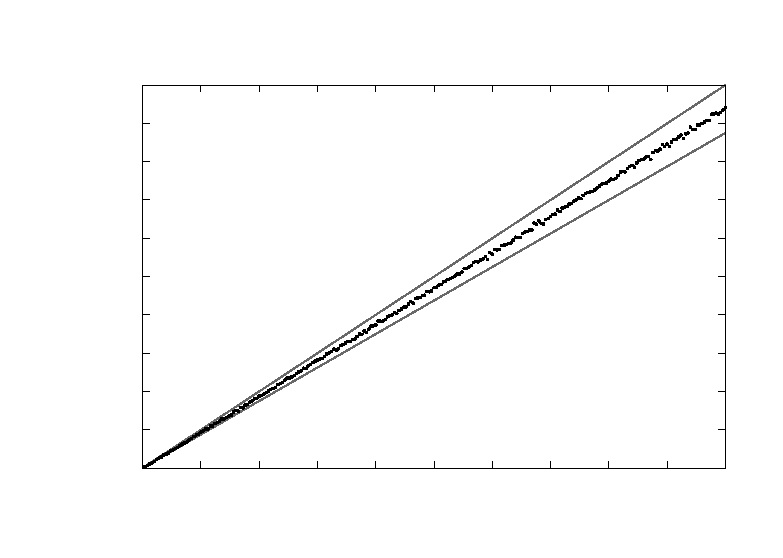
\includegraphics{build}}%
    \gplfronttext
  \end{picture}%
\endgroup

     \caption{\small \sl Results of build heap algorithm.\label{fig:build}}  
\end{center}
\end{figure}

\begin{figure}[h]
\begin{center}
 \begin{tabular}{||c | c | c||} 
 \hline
 Depth of Nodes &  Height of Nodes & Num. of Comparisons \\ [0.5ex] 
 \hline
 \hline
 $h$ & 0 & 0 \\
 \hline 
 
 $h-1$ & 1 & $2(\frac{n}{4})$  \\ 
 \hline
 
 $h-2$ & 2 & $2(\frac{n}{8} + \frac{n}{4})$  \\
 \hline
 
 $h-3$ & 3 & $2(\frac{n}{16} + \frac{n}{8} + \frac{n}{4})$   \\
 \hline
 
 ... & ... & ...  \\
 \hline
\end{tabular}
\end{center}
\caption{\small \sl Breakdown of total comparisons by height of heap, in worst-case. \label{fig:tab}}
\end{figure}

At first glance, it would appear that the algorithm is described by $O(n \log n)$ since there is a single deterministic loop that iterates $\frac{n}{2} - 1$ times containing a $O(\log n)$ method. This is technically correct, but not the most optimal analysis. Upon closer inspection we can tighten the bound to $\Theta(n)$ because \method{percolate_down} is only $\Omega(1)$ for a single run, but, over multiple runs of a heap it is shown to be $\Theta(\log n)$ \cite{aocp}.

In the \method{build_heap} algorithm, an arbitrary heap is created, followed by \method{percolate_down} being called in reverse level order starting on the first parent node. The total number of comparisons in a worst-case \method{build_heap} scenario is shown in Figure \ref{fig:tab}. We observe that nodes of height 0 (there are $\frac{n}{2}$) have 0 comparisons because they have no children, and the total number of comparisons in \method{build_heap} can be represented as the summation shown below.
\[
	\sum_{i=1}^{h}\frac{2(n+1)}{2^{i+1}} \in O(n)
\]


This summation can be shown to be linear \cite{beck}, and after observing that the algorithm must access every element of the heap at least once, we can see the \method{build_heap} is $\Omega(n)$ time. Therefore, we conclude that the algorithm is of the form
\[
	T(n)\in \Theta(n)
\]
The author never explicitly states what efficiency class the algorithm is in, but it can be assumed that they concluded that it is $O(n)$ \cite[230]{levit}. Our analysis does agree with the author's, up to a point, but by observing that the algorithm must be at least $\Omega(n)$ we can tighten our bound to Big-$\Theta$, instead of just Big-$O$.

\section{Heapsort}

In general, a heapsort algorithm contains two major parts: building the heap from data and repeatedly removing the highest valued node to put into the to-be-sorted array.
%
To analyze the \method{heap_sort} algorithm we chose the \method{delete_max()} method  on line 123 as the basic operation because this occurs most frequently and is the philosophical heart of this algorithm. We ruled out building the heap since it only occurs once, and was shown previously to be $\Theta(n)$.

\begin{center}
    % GNUPLOT: LaTeX picture with Postscript
\begingroup
  \makeatletter
  \providecommand\color[2][]{%
    \GenericError{(gnuplot) \space\space\space\@spaces}{%
      Package color not loaded in conjunction with
      terminal option `colourtext'%
    }{See the gnuplot documentation for explanation.%
    }{Either use 'blacktext' in gnuplot or load the package
      color.sty in LaTeX.}%
    \renewcommand\color[2][]{}%
  }%
  \providecommand\includegraphics[2][]{%
    \GenericError{(gnuplot) \space\space\space\@spaces}{%
      Package graphicx or graphics not loaded%
    }{See the gnuplot documentation for explanation.%
    }{The gnuplot epslatex terminal needs graphicx.sty or graphics.sty.}%
    \renewcommand\includegraphics[2][]{}%
  }%
  \providecommand\rotatebox[2]{#2}%
  \@ifundefined{ifGPcolor}{%
    \newif\ifGPcolor
    \GPcolorfalse
  }{}%
  \@ifundefined{ifGPblacktext}{%
    \newif\ifGPblacktext
    \GPblacktexttrue
  }{}%
  % define a \g@addto@macro without @ in the name:
  \let\gplgaddtomacro\g@addto@macro
  % define empty templates for all commands taking text:
  \gdef\gplbacktext{}%
  \gdef\gplfronttext{}%
  \makeatother
  \ifGPblacktext
    % no textcolor at all
    \def\colorrgb#1{}%
    \def\colorgray#1{}%
  \else
    % gray or color?
    \ifGPcolor
      \def\colorrgb#1{\color[rgb]{#1}}%
      \def\colorgray#1{\color[gray]{#1}}%
      \expandafter\def\csname LTw\endcsname{\color{white}}%
      \expandafter\def\csname LTb\endcsname{\color{black}}%
      \expandafter\def\csname LTa\endcsname{\color{black}}%
      \expandafter\def\csname LT0\endcsname{\color[rgb]{1,0,0}}%
      \expandafter\def\csname LT1\endcsname{\color[rgb]{0,1,0}}%
      \expandafter\def\csname LT2\endcsname{\color[rgb]{0,0,1}}%
      \expandafter\def\csname LT3\endcsname{\color[rgb]{1,0,1}}%
      \expandafter\def\csname LT4\endcsname{\color[rgb]{0,1,1}}%
      \expandafter\def\csname LT5\endcsname{\color[rgb]{1,1,0}}%
      \expandafter\def\csname LT6\endcsname{\color[rgb]{0,0,0}}%
      \expandafter\def\csname LT7\endcsname{\color[rgb]{1,0.3,0}}%
      \expandafter\def\csname LT8\endcsname{\color[rgb]{0.5,0.5,0.5}}%
    \else
      % gray
      \def\colorrgb#1{\color{black}}%
      \def\colorgray#1{\color[gray]{#1}}%
      \expandafter\def\csname LTw\endcsname{\color{white}}%
      \expandafter\def\csname LTb\endcsname{\color{black}}%
      \expandafter\def\csname LTa\endcsname{\color{black}}%
      \expandafter\def\csname LT0\endcsname{\color{black}}%
      \expandafter\def\csname LT1\endcsname{\color{black}}%
      \expandafter\def\csname LT2\endcsname{\color{black}}%
      \expandafter\def\csname LT3\endcsname{\color{black}}%
      \expandafter\def\csname LT4\endcsname{\color{black}}%
      \expandafter\def\csname LT5\endcsname{\color{black}}%
      \expandafter\def\csname LT6\endcsname{\color{black}}%
      \expandafter\def\csname LT7\endcsname{\color{black}}%
      \expandafter\def\csname LT8\endcsname{\color{black}}%
    \fi
  \fi
    \setlength{\unitlength}{0.0500bp}%
    \ifx\gptboxheight\undefined%
      \newlength{\gptboxheight}%
      \newlength{\gptboxwidth}%
      \newsavebox{\gptboxtext}%
    \fi%
    \setlength{\fboxrule}{0.5pt}%
    \setlength{\fboxsep}{1pt}%
\begin{picture}(7200.00,5040.00)%
    \gplgaddtomacro\gplbacktext{%
      \csname LTb\endcsname%
      \put(1210,704){\makebox(0,0)[r]{\strut{}$0$}}%
      \put(1210,1317){\makebox(0,0)[r]{\strut{}$20000$}}%
      \put(1210,1929){\makebox(0,0)[r]{\strut{}$40000$}}%
      \put(1210,2542){\makebox(0,0)[r]{\strut{}$60000$}}%
      \put(1210,3154){\makebox(0,0)[r]{\strut{}$80000$}}%
      \put(1210,3767){\makebox(0,0)[r]{\strut{}$100000$}}%
      \put(1210,4379){\makebox(0,0)[r]{\strut{}$120000$}}%
      \put(1342,484){\makebox(0,0){\strut{}$0$}}%
      \put(1888,484){\makebox(0,0){\strut{}$500$}}%
      \put(2434,484){\makebox(0,0){\strut{}$1000$}}%
      \put(2980,484){\makebox(0,0){\strut{}$1500$}}%
      \put(3526,484){\makebox(0,0){\strut{}$2000$}}%
      \put(4073,484){\makebox(0,0){\strut{}$2500$}}%
      \put(4619,484){\makebox(0,0){\strut{}$3000$}}%
      \put(5165,484){\makebox(0,0){\strut{}$3500$}}%
      \put(5711,484){\makebox(0,0){\strut{}$4000$}}%
      \put(6257,484){\makebox(0,0){\strut{}$4500$}}%
      \put(6803,484){\makebox(0,0){\strut{}$5000$}}%
      \put(2980,1720){\rotatebox{31}{\makebox(0,0)[l]{\strut{}$\frac{5}{2} n\log n$}}}%
      \put(3526,1480){\rotatebox{27}{\makebox(0,0)[l]{\strut{}$2n \log n$}}}%
    }%
    \gplgaddtomacro\gplfronttext{%
      \csname LTb\endcsname%
      \put(176,2541){\rotatebox{-270}{\makebox(0,0){\strut{}Operation Count}}}%
      \put(4072,154){\makebox(0,0){\strut{}Input Size}}%
      \put(4072,4709){\makebox(0,0){\strut{}\textbf{Empirical Analysis of Heap Sort Algorithm}}}%
    }%
    \gplbacktext
    \put(0,0){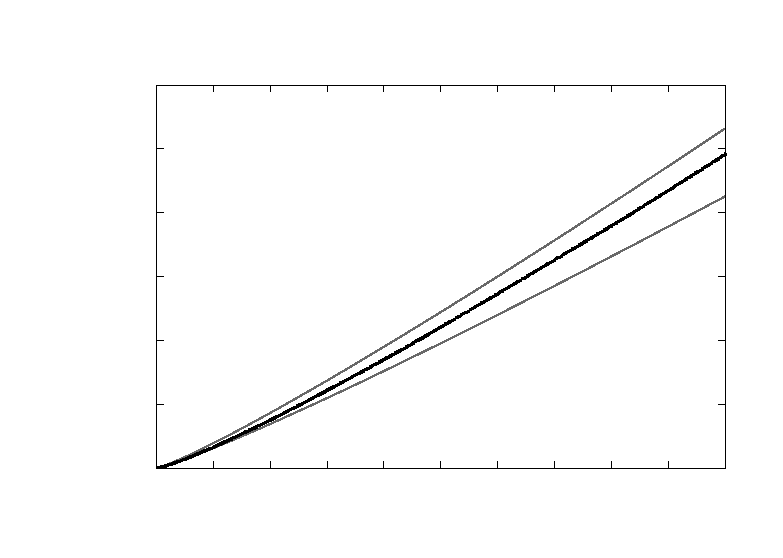
\includegraphics{sort}}%
    \gplfronttext
  \end{picture}%
\endgroup

        \captionof{figure}{Results of implemented heapsort algorithm.}
        \label{fig:sort}
\end{center}

An empirical analysis of running \method{heap_sort} for multiple values of $n$ produces the results shown above, in Figure \ref{fig:sort}. The standard function $f(n) = n \log n$ with constant multipliers, has been added to illustrate the analysis.

An examination of the code itself explains the empirical results when we observe that this algorithm uses the method \method{delete_max()}, which deletes the largest valued node and \textit{re-heaps} the heap using \method{percolate_down}. Since this method call is in a deterministic for loop and \method{delete_max}'s basic operation was shown to be $\Theta(\log n)$ time, we can extrapolate that \method{heap_sort} is of the form
\[
	T(n)\in \Theta(n\log n)
\]

However, this analysis is completely dependent upon one thing: the input data. The best case scenario depends wholly upon the whether or not the data has duplicate values in it. If there are duplicate values in the data the best-case runtime turns into $\Omega(n)$, however, if duplicates do not appear in the data then the best-case runtime turns into $\Omega(n\log n)$ \cite[84--86]{anal}.

Shown below are possible conclusions based on input data.

\textbf{Duplicates}
\[
	T(n)\in O(n\log n)
	\]
	\[
	T(n)\in \Omega(n)
	\]
\textbf{Unique}
\[
	T(n)\in \Theta(n\log n)
\]

Our author states `` [heapsort] falls in the same class as that of mergesort'', which is not an outright conclusion, but points toward the assumption of $\Theta(n \log n)$. Our analysis agrees with our author's conclusion only if the data does not include duplicates. If the data does include duplicates the only thing affected is the algorithm's best-case, and thus changes our Big-$\Theta$ to Big-$O$.
\nocite{*}
\clearpage
\printbibliography

\end{document}